\section*{Пешеходная библиотека}
\addcontentsline{toc}{section}{Пешеходная библиотека}
\subsection*{Пешеходная библиотека. Первая модель}
\addcontentsline{toc}{subsection}{Пешеходная библиотека. Первая модель}

\textbf{Задание:}\\
Разработать модель движения пассажиров в наземном павильоне метро.\\

\textbf{Решение:}\\
Перед тем, как пройти к поездам метро, пассажиры проходят через турникеты, проверяющие наличие проездного документа. Некоторые пассажиры должны будут вначале приобрести жетоны или проездные билеты в кассе.\\

На первом шаге необходимо разметить пространство, а именно -- отрисовать стены, целевые линии, которые указывают вход и выход из модели, разместить сервисы с очередями, чтобы обозначить турникеты и кассы. (Рисунок \ref{fig:simple_metro1})
\begin{figure}[h]
	\centering 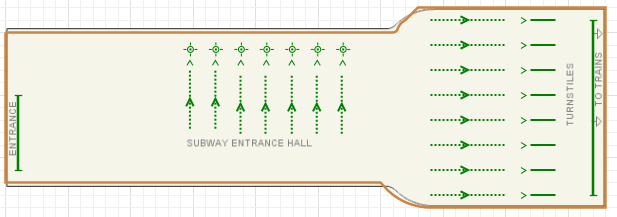
\includegraphics[scale=0.3]{simple_metro1}
	\caption{Разметка пространства наземного павильона метро}
	\label{fig:simple_metro1}
\end{figure}

Далее была разработана основная логика модели. (Рисунок \ref{fig:simple_metro2})
\begin{figure}[h]
	\centering 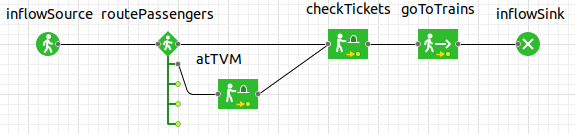
\includegraphics[scale=0.5]{simple_metro2}
	\caption{Описание логики модели}
	\label{fig:simple_metro2}
\end{figure}

\newpage

Агенты поступают в модель согласно заданной интенсивности, затем у них есть выбор либо пойти в кассы и купить билет, либо сразу пойти к турникетам. Выбор осуществляется на основе заданной вероятности в 70\%. (Рисунок \ref{fig:simple_metro3})
\begin{figure}[h]
	\centering 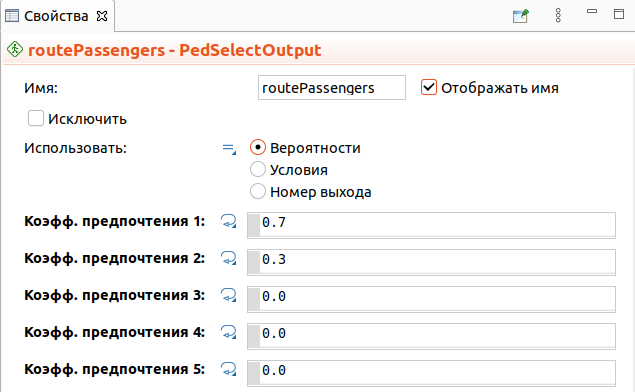
\includegraphics[scale=0.4]{simple_metro3}
	\caption{Принятие решения в модели}
	\label{fig:simple_metro3}
\end{figure}

Блоки обслуживания агентов задаются идентичным образом как это было в Библиотеке моделирования процессов. Выход из модели осуществляется путём достижения линии выхода.\\

Для отслеживания возникновения мест с большим скоплением агентов используем карту плотности, тогда модель будет выглядеть следующим образом. (Рисунок \ref{fig:simple_metro4})
\begin{figure}[h]
	\centering 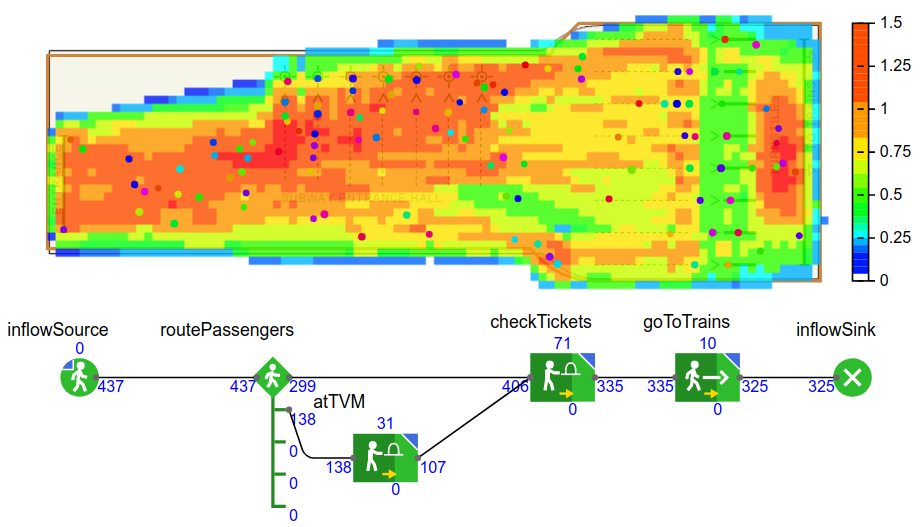
\includegraphics[scale=0.35]{simple_metro4}
	\caption{Принятие решения в модели}
	\label{fig:simple_metro4}
\end{figure}

Таким образом, на примере модели метро, нами был рассмотрен инструментарий пешеходной библиотеки.\\